% !TEX root =../dissertation.tex
\documentclass[./dissertation.tex]{subfiles}

\begin{document}
% \chapter{A Novel Pipeline for Cell Instance Segmentation, Tracking and Motility Classification of Toxoplasma Gondii in 3D Space}
\chapter{Deep Models For Supervised Image Segmentation}
\label{ch:toxo}

% Toxoplasma gondii is the parasitic protozoan that causes disseminated toxoplasmosis, a disease that is estimated to infect around one-third of the world's population. While the disease is commonly asymptomatic, the success of the parasite is in large part due to its ability to easily spread through nucleated cells. The virulence of T. gondii is predicated on the parasite's motility. Thus the inspection of motility patterns during its lytic cycle has become a topic of keen interest. Current cell tracking projects usually focus on cell images captured in 2D which are not a true representation of the actual motion of a cell. Current 3D tracking projects lack a comprehensive pipeline covering all phases of preprocessing, cell detection, cell instance segmentation, tracking, and motion classification, and merely implement a subset of the phases. Moreover, current 3D segmentation and tracking pipelines are not targeted for users with less experience in deep learning packages. Our pipeline, TSeg, on the other hand, is developed for segmenting, tracking, and classifying the motility phenotypes of T. gondii in 3D microscopic images. Although TSeg is built initially focusing on T. gondii, it provides generic functions to allow users with similar but distinct applications to use it off-the-shelf. Interacting with all of TSeg's modules is possible through our Napari plugin which is developed mainly off the familiar SciPy scientific stack. Additionally, our plugin is designed with a user-friendly GUI in Napari which adds several benefits to each step of the pipeline such as visualization and representation in 3D. TSeg proves to fulfill a better generalization, making it capable of delivering accurate results with images of other cell types.
% \chapter{A Novel Pipeline for Cell Instance Segmentation, Tracking and Motility Classification of \textit{Toxoplasma gondii} in 3D Space}

\section{Introduction}
Quantitative cell research often requires the measurement of different cell properties including size, shape, and motility. This step is facilitated using segmentation of imaged cells. With fluorescent markers, computational tools can be used to complete segmentation and identify cell features and positions over time. 2D measurements of cells can be useful, but the more difficult task of deriving 3D information from cell images is vital for metrics such as motility and volumetric qualities.

Most of the state-of-the-art pipelines are restricted to 2D space which is not a true representative of the actual motion of the organism. Many of them require knowledge and expertise in programming, or in machine learning and deep learning models and frameworks, thus limiting the demographic of users that can use them. All of them solely include a subset of the aforementioned modules (i.e. detection, segmentation, tracking, and classification) \cite{stringer2021cellpose}. Many pipelines rely on the user to train their own model, hand-tailored for their specific application. This demands high levels of experience and skill in ML/DL and consequently undermines the possibility and feasibility of quickly utilizing an off-the-shelf pipeline and still getting good results. PlantSeg uses a variant of 3D U-Net, called Residual 3D U-Net, for preprocessing and segmentation of multiple cell types \cite{plantseg}. PlantSeg performs best among Deep Learning algorithms for 3D Instance Segmentation and is very robust against image noise \cite{Kar2021.06.09.447748}. The segmentation module also includes the optional use of CellPose \cite{stringer2021cellpose}. CellPose is a generalized segmentation algorithm trained on a wide range of cell types and is the first step toward increased optionality in TSeg. The Cell Tracking module consolidates the cell particles across the z-axis to materialize cells in 3D space and estimates centroids for each cell. The tracking module is also responsible for extracting the trajectories of cells based on the movements of centroids throughout consecutive video frames, which is eventually the input of the motion classifier module.

Toxoplasmosis is an infection caused by the intracellular parasite \textit{Toxoplasma gondii}. (\textit{T. gondii}) is one of the most successful parasites, infecting at least one-third of the world's population. Although Toxoplasmosis is generally benign in healthy individuals, the infection has fatal implications in fetuses and immunocompromised individuals \cite{saadatnia2012review}. \textit{T. gondii}'s virulence is directly linked to its lytic cycle which is comprised of invasion, replication, egress, and motility. Studying the motility of \textit{T. gondii} is crucial in understanding its lytic cycle in order to develop potential treatments.

To address these we present TSeg. It segments \textit{T. gondii} cells in 3D microscopic images, tracks their trajectories, and classifies the motion patterns observed throughout the 3D frames. TSeg is comprised of four modules: pre-processing, segmentation, tracking, and classification. We developed TSeg as a plugin for Napari \cite{sofroniew_nicholas_2022_6598542} - an open-source fast and interactive image viewer for Python designed for browsing, annotating, and analyzing large multi-dimensional images. Having TSeg implemented as a part of Napari not only provides a user-friendly design but also gives more advanced users the possibility to attach and execute their custom code and even interact with the steps of the pipeline if needed. The preprocessing module is equipped with basic and extra filters and functionalities to aid in the preparation of the input data. TSeg gives its users the advantage of utilizing the functionalities that PlantSeg and CellPose provide. These functionalities can be chosen in the pre-processing, detection, and segmentation steps. This brings forth a huge variety of algorithms and pre-built models to select from, making TSeg not only a great fit for T. gindii, but also a variety of different cell types.

% For this reason, we present a novel pipeline to detect, segment, track, and classify the motility pattern of \textit{T. gondii} in 3D space. One of the main goals is to make our pipeline intuitively easy to use so that the users who are not experienced in the fields of machine learning (ML), deep learning (DL), or computer vision (CV) can still benefit from it. The other objective is to equip it with the most robust and accurate set of segmentation and detection tools so that the end product has a broad generalization, allowing it to perform well and accurately for various cell types right off the shelf.


% \textit{Toxoplasma gondii} is the parasitic protozoan that causes disseminated toxoplasmosis, a disease that is estimated to infect around one-third of the world's population. While the disease is commonly asymptomatic, the success of the parasite is in large part due to its ability to easily spread through nucleated cells. The virulence of \textit{T. gondii} is predicated on the parasite's motility. Thus the inspection of motility patterns during its lytic cycle has become a topic of keen interest. Current cell tracking projects usually focus on cell images captured in 2D which are not a true representation of the actual motion of a cell. Current 3D tracking projects lack a comprehensive pipeline covering all phases of preprocessing, cell detection, cell instance segmentation, tracking, and motion classification, and merely implement a subset of the phases. Moreover, current 3D segmentation and tracking pipelines are not targeted for users with less experience in deep learning packages. Our pipeline, TSeg, on the other hand, is developed for segmenting, tracking, and classifying the motility phenotypes of \textit{T. gondii} in 3D microscopic images. Although TSeg is built initially focusing on \textit{T. gondii}, it provides generic functions to allow users with similar but distinct applications to use it off-the-shelf. Interacting with all of TSeg's modules is possible through our Napari plugin which is developed mainly off the familiar SciPy scientific stack. Additionally, our plugin is designed with a user-friendly GUI in Napari which adds several benefits to each step of the pipeline such as visualization and representation in 3D. TSeg proves to fulfill a better generalization, making it capable of delivering accurate results with images of other cell types.







\section{Background}

The recent solutions in generalized and automated segmentation tools are focused on 2D cell images. Segmentation of cellular structures in 2D is important but not representative of realistic environments. Microbiological organisms are free to move on the z-axis and tracking without taking this factor into account cannot guarantee a full representation of the actual motility patterns. As an example, Fazli et al. \cite{fazli2018unsupervised} identified three distinct motility types for \textit{T. gondii} with two-dimensional data, however, they also acknowledge and state that based established heuristics from previous works there are more than three motility phenotypes for \textit{T. gondii}. The focus on 2D research is understandable due to several factors. 3D data is difficult to capture as tools for capturing 3D slices and the computational requirements for analyzing this data are not available in most research labs. Most segmentation tools are unable to track objects in 3D space as the assignment of related centroids is more difficult. The additional noise from capture and focus increases the probability of incorrect assignment. 3D data also has issues with overlapping features and increased computation required per frame of time.

Fazli et al. \cite{fazli2018unsupervised} studies the motility patterns of \textit{T. gondii} and provides a computational pipeline for identifying motility phenotypes of \textit{T. gondii} in an unsupervised, data-driven way. In that work Ca2+ is added to \textit{T. gondii} cells inside a Fetal Bovine Serum. \textit{T. gondii} cells react to Ca2+ and become motile and fluorescent. The images of motile \textit{T. gondii} cells were captured using an LSM 710 confocal microscope. They use Python 3 and associated scientific computing libraries (NumPy, SciPy, scikit-learn, matplotlib) in their pipeline to track and cluster the trajectories of \textit{T. gondii}. Based on this work Fazli et al. \cite{fazli2018toward} work on another pipeline consisting of preprocessing, sparsification, cell detection, and cell tracking modules to track \textit{T. gondii} in 3D video microscopy where each frame of the video consists of image slices taken 1 micro-meters of focal depth apart along the z-axis direction. In their latest work Fazli et al. \cite{fazli2019lightweight} developed a lightweight and scalable pipeline using task distribution and parallelism. Their pipeline consists of multiple modules: reprocessing, sparsification, cell detection, cell tracking, trajectories extraction, parametrization of the trajectories, and clustering. They could classify three distinct motion patterns in \textit{T. gondii} using the same data from their previous work.

While combining open-source tools is not a novel architecture, little has been done to integrate 3D cell tracking tools. Fazeli et al. \cite{fazeli2020automated}, motivated by the interest in providing robust yet accessible tools for researchers without programming expertise, developed a comprehensive pipeline combining StarDist \cite{Weigert_2020} and TrackMate \cite{TINEVEZ201780} for automated 2D cell tracking. This pipeline leverages the ZeroCostDL4Mic \cite{von2021democratising} platform, enabling researchers with no coding experience to train deep learning models on their own data, significantly lowering the barrier to entry. StarDist facilitates segmentation with star-convex polygon approximation, robustly distinguishing cells from the background even in challenging imaging conditions. TrackMate then uses these segmentation outputs to reliably track cells across timeframes, providing quantitative analytics such as velocity and trajectory characteristics. Despite its utility, the pipeline remains limited to 2D analysis, highlighting the need for extending such integrative approaches to 3D microscopy, as we propose with TSeg.

This Stardist pipeline is similar in concept to TSeg. Both create an automated segmentation and tracking pipeline but TSeg is oriented to 3D data. Cells move in 3-dimensional space that is not represented in a flat plane. TSeg also does not require the manual training necessary for the other pipeline. Individuals with low technical expertise should not be expected to create masks for training or even understand the training of deep neural networks. Lastly, this pipeline does not account for imperfect datasets without the need for preprocessing. All implemented algorithms in TSeg account for microscopy images with some amount of noise.

Wen et al. \cite{Wen2021-bn} combines multiple existing new technologies including deep learning and presents 3DeeCellTracker. 3DeeCellTracker segments and tracks cells on 3D time-lapse images. Using a small subset of their dataset they train the deep learning architecture 3D U-Net for segmentation. For tracking, a combination of two strategies was used to increase accuracy: local cell region strategies, and spatial pattern strategy. Kapoor et al. \cite{kapoor2021cell} presents VollSeg that uses deep learning methods to segment, track, and analyze cells in 3D with irregular shape and intensity distribution. It is a Jupyter Notebook-based Python package and also has a UI in Napari. For tracking, a custom tracking code is developed based on Trackmate.

Many segmentation tools require some amount of knowledge in Machine or Deep Learning concepts. Training the neural network in creating masks is a common step for open-source segmentation tools. Automating this process makes the pipeline more accessible to microbiology researchers.

\section{Methodologies}
\subsection{Data}
Our dataset consists of 11 videos of \textit{\textit{T. gondii}} cells under a microscope, obtained from different experiments with different numbers of cells. The videos are on average around 63 frames in length. Each frame has a stack of 41 image slices of size 500×502 pixels along the z-axis (z-slices). The z-slices are captured 1µm apart in optical focal length making them 402µm×401µm×40µm in volume. The slices were recorded in raw format as RGB TIF images but are converted to grayscale for our purpose. This data is captured using a PlanApo 20x objective (NA = 0.75) on a preheated Nikon Eclipse TE300 epifluorescence microscope. The image stacks were captured using an iXon 885 EMCCD camera (Andor Technology, Belfast, Ireland) cooled to -70°C and driven by NIS Elements software (Nikon Instruments, Melville, NY) as part of related research by Ward et al. \cite{TgPHIL1}. The camera was set to frame transfer sensor mode, with a vertical pixel shift speed of 1.0 µs, vertical clock voltage amplitude of +1, readout speed of 35MHz, conversion gain of 3.8×, EM gain setting of 3 and 2×2 binning, and the z-slices were imaged with an exposure time of 16ms.

\subsection{Software}
\subsubsection{Napari Plugin}
TSeg is developed as a plugin for Napari - a fast and interactive multi-dimensional image viewer for Python that allows volumetric viewing of 3D images \cite{sofroniew_nicholas_2022_6598542}. Plugins enable developers to customize and extend the functionality of Napari. For every module of TSeg, we developed its corresponding widget in the GUI, plus a widget for file management. The widgets have self-explanatory interface elements with tooltips to guide the inexperienced user to traverse through the pipeline with ease. Layers in Napari are the basic viewable objects that can be shown in the Napari viewer. Seven different layer types are supported in Napari: Image, Labels, Points, Shapes, Surface, Tracks, and Vectors, each of which corresponds to a different data type, visualization, and interactivity \cite{sofroniew_nicholas_2022_6598542}. After its execution, the viewable output of each widget gets added to the layers. This allows the user to evaluate and modify the parameters of the widget to get the best results before continuing to the next widget. Napari supports bidirectional communication between the viewer and the Python kernel and has a built-in console that allows users to control all the features of the viewer programmatically. This adds more flexibility and customizability to TSeg for the advanced user. The full code of TSeg is available on GitHub under the MIT open source license at \url{https://github.com/salirezav/tseg}. TSeg can be installed through Napari's plugins menu.

\begin{figure}[h]
    \centering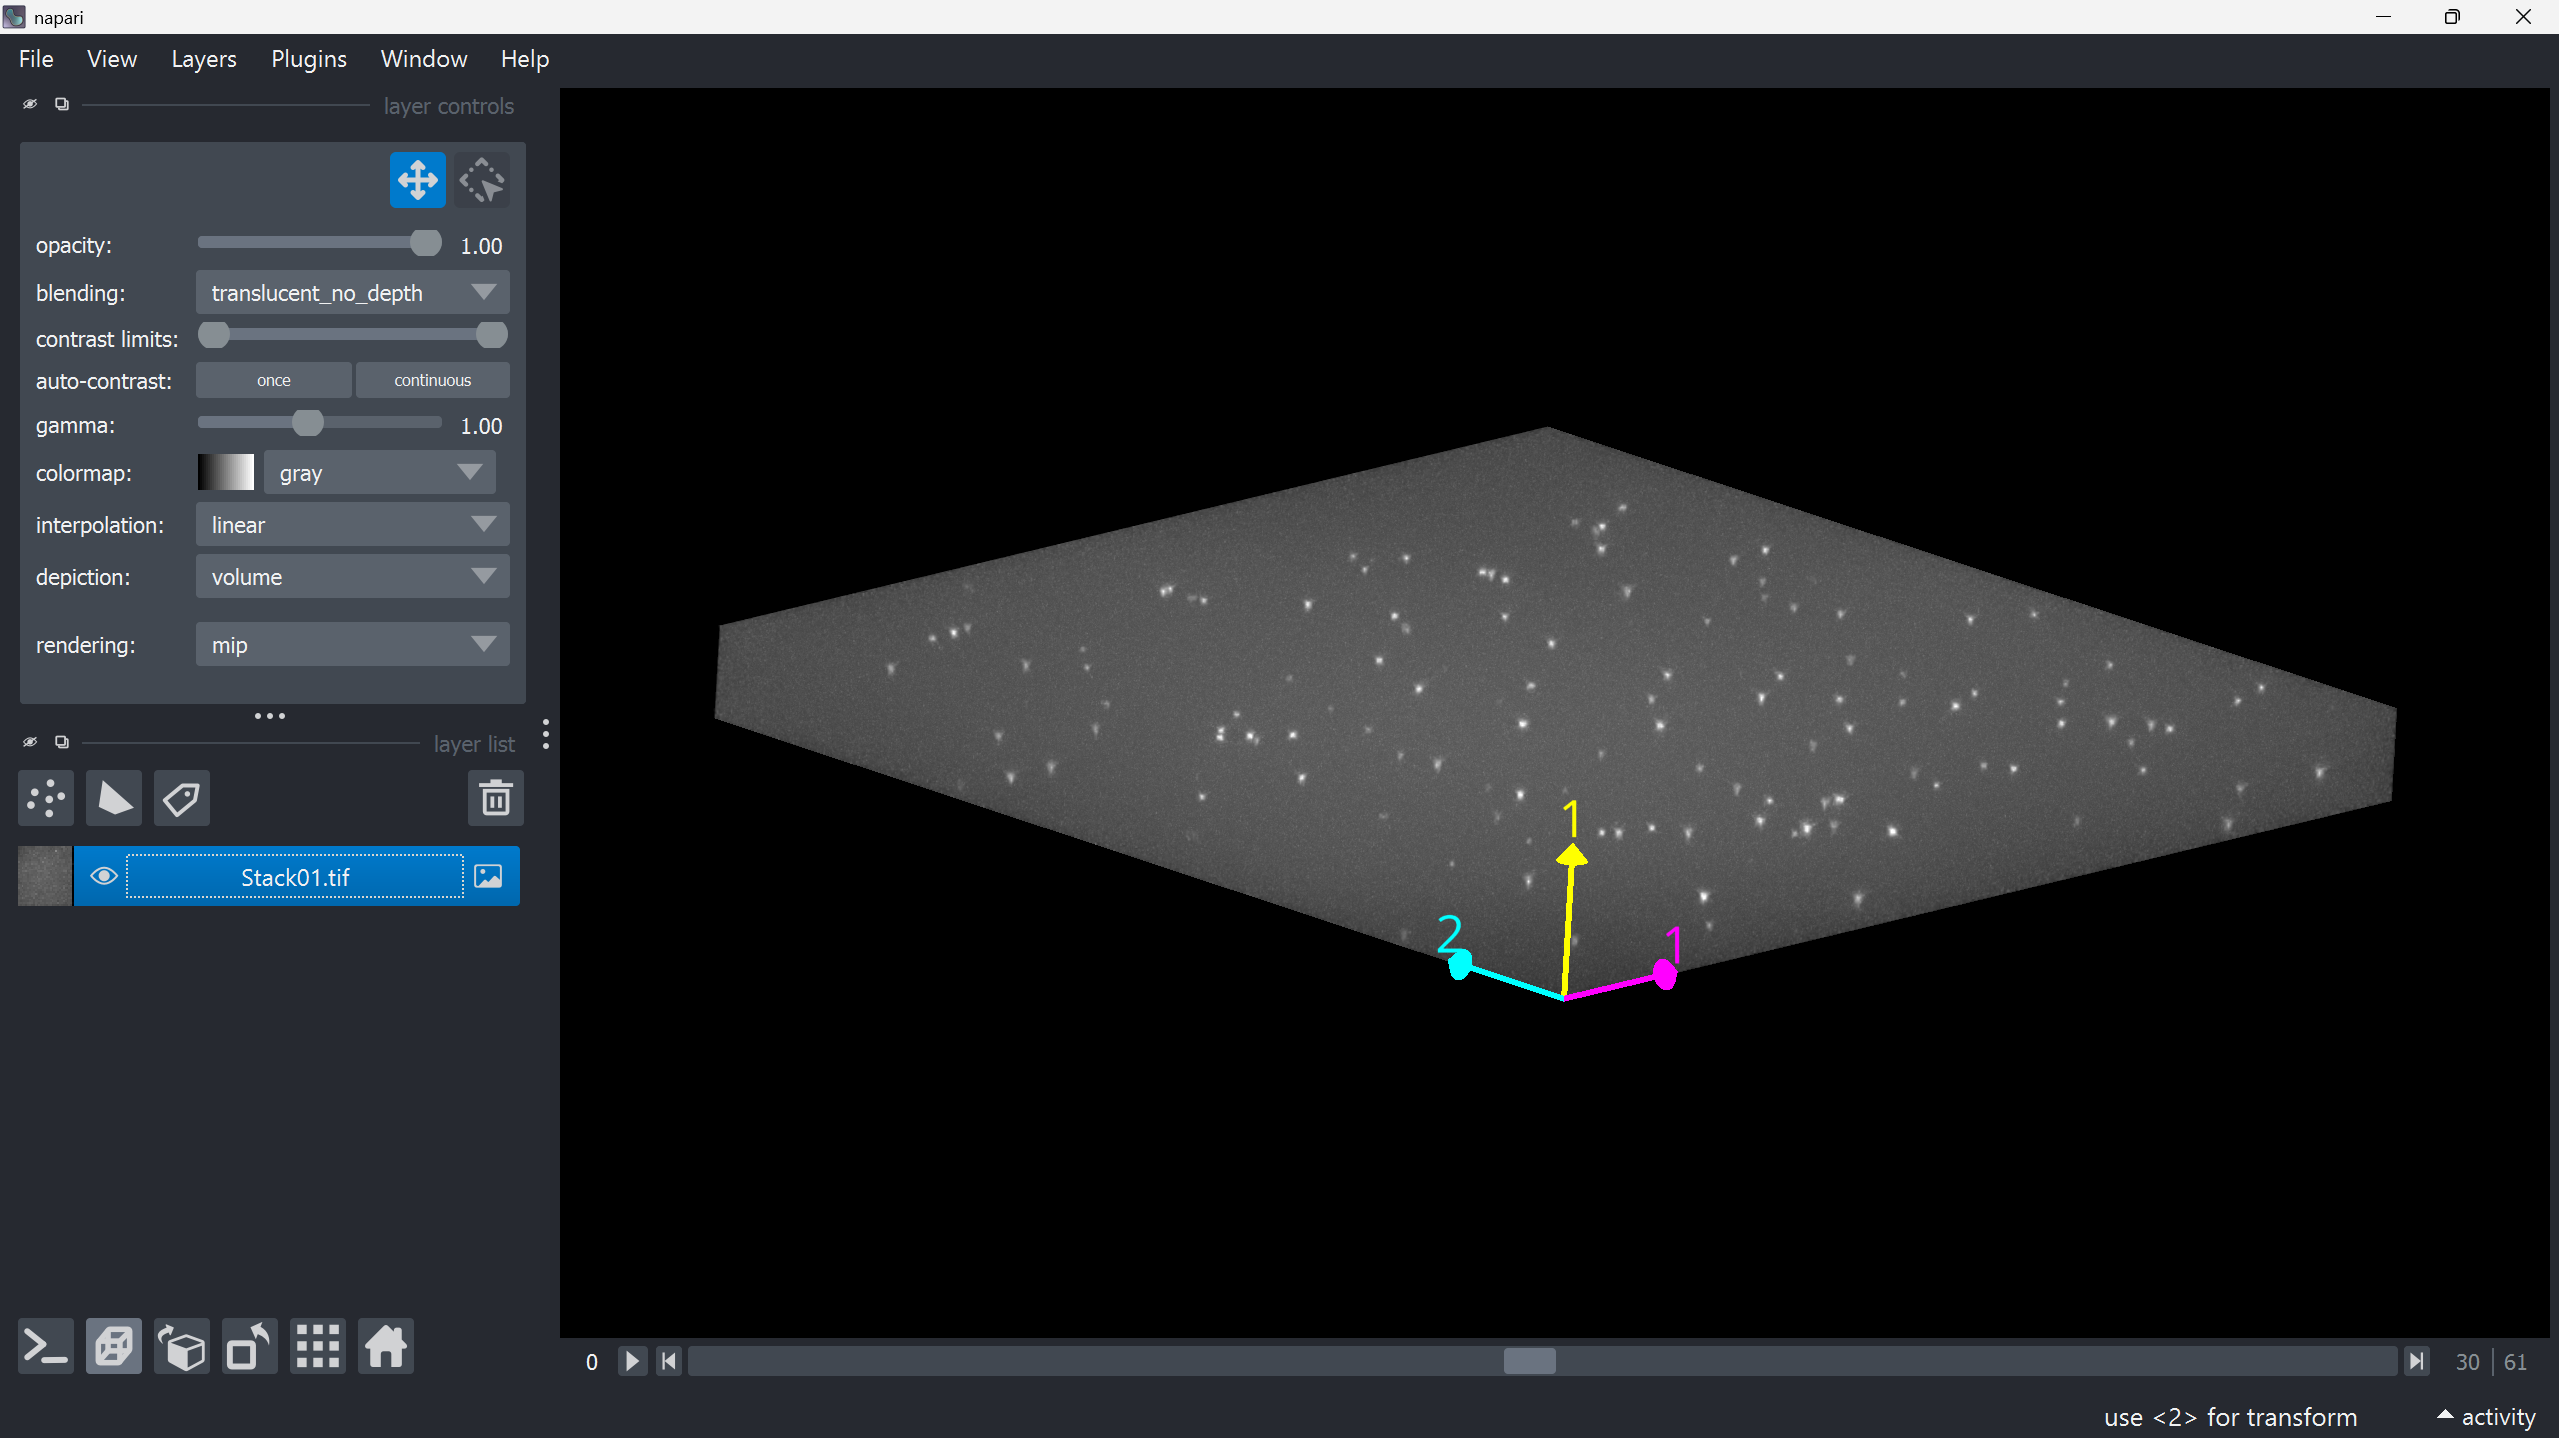
\includegraphics[width=.8\textwidth]{figures/tseg/3d viewer.png}
    \caption{TSeg's Napari Plugin Interface}
    \label{fig:viewer}
\end{figure}





\subsubsection{Computational Pipeline}
\textbf{Pre-Processing} \\
Due to the fast imaging speed in data acquisition, the image slices will inherently have a vignetting artifact, meaning that the corners of the images will be slightly darker than the center of the image - Figure \ref{fig:raw_toxo}. To eliminate this artifact we added adaptive thresholding and logarithmic correction to the pre-processing module. Furthermore, another prevalent artifact on our dataset images was a Film-Grain noise (AKA salt and pepper noise). To remove or reduce such noise a simple gaussian blur filter and a sharpening filter are included.

\begin{figure}[h]
    \centering\includegraphics[width=.3\textwidth]{figures/tseg/rax toxo.png}
    \centering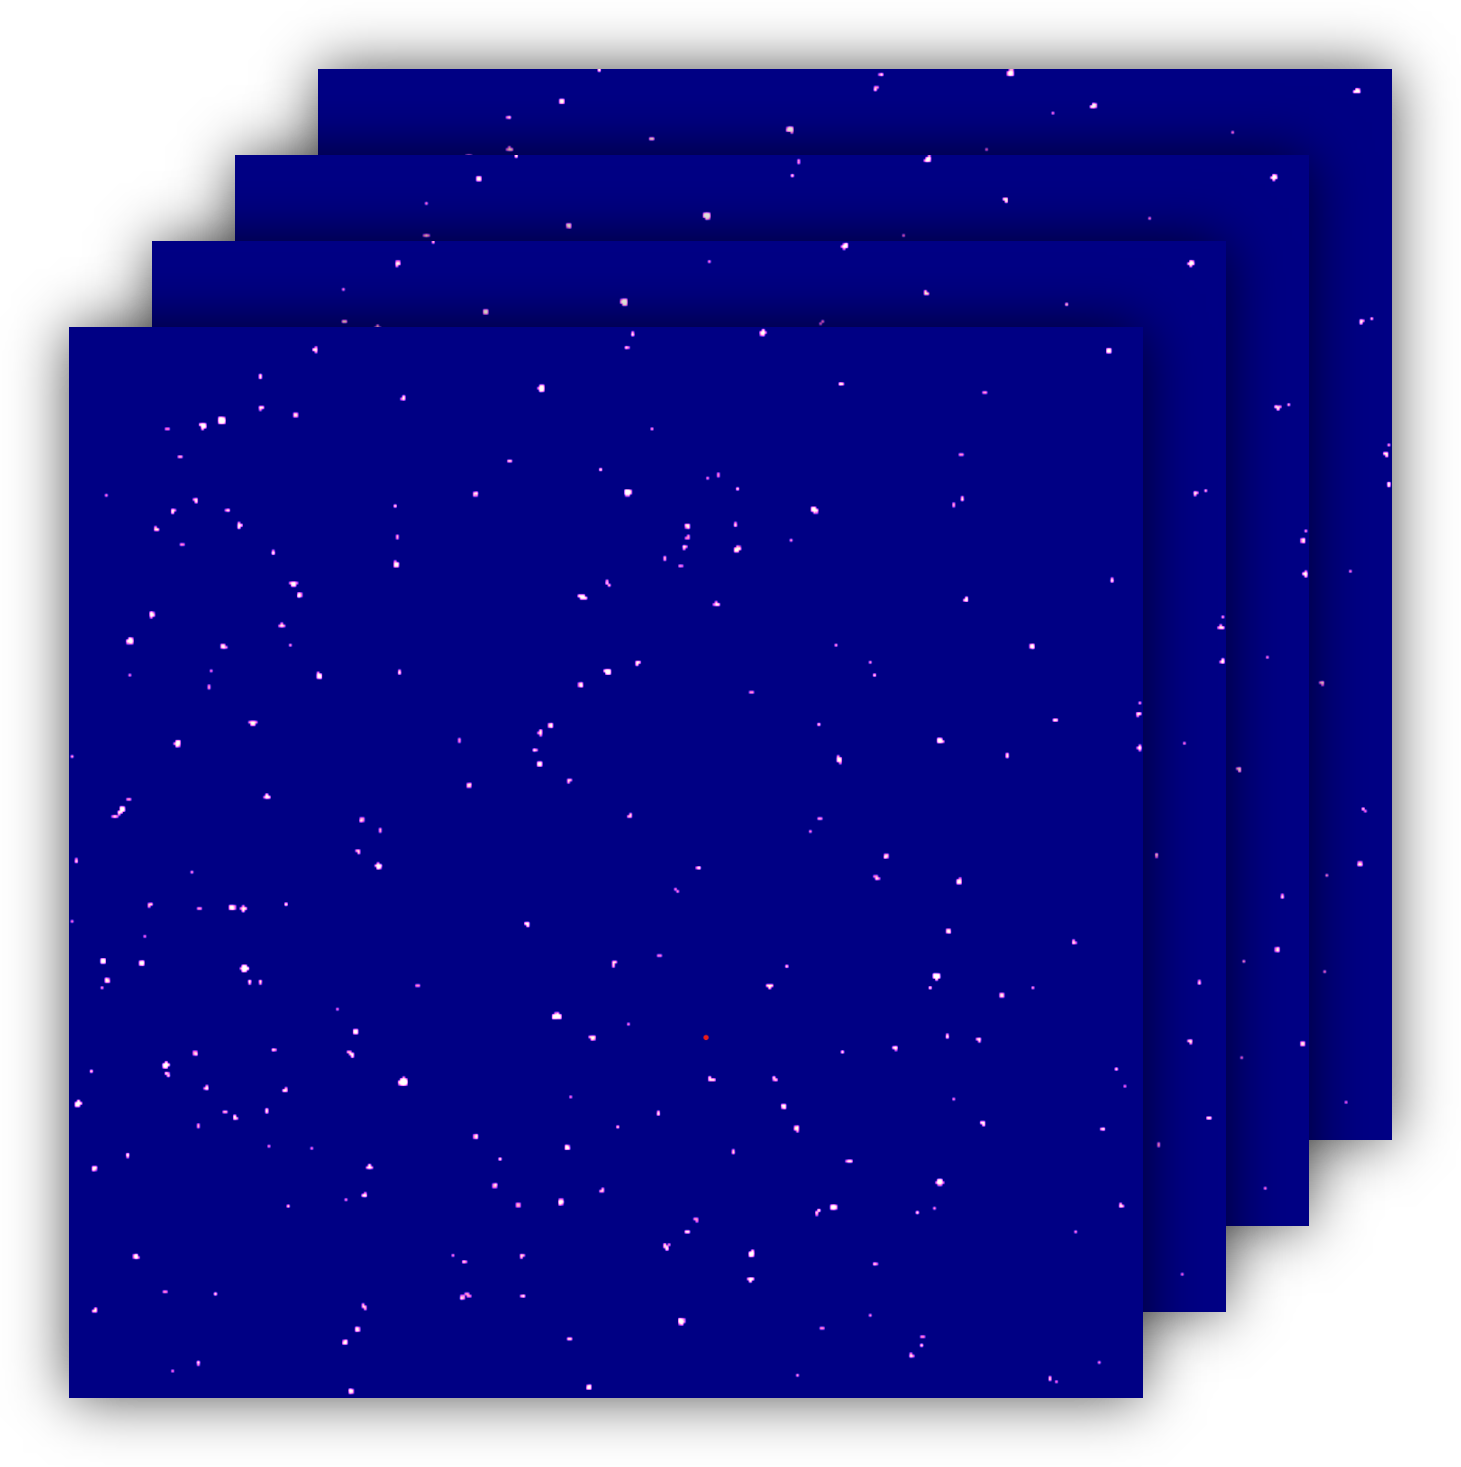
\includegraphics[width=.3\textwidth]{figures/tseg/denoised.png}
    \caption{On the left, a sample frame of the 3D video of \textit{\textit{T. gondii}} cells. The image is captured using a PlanApo 20x objective (NA = 0.75) on a preheated Nikon Eclipse TE300 epifluorescence microscope. On the right, the same frame after denoising.}
    \label{fig:raw_toxo}
\end{figure}


\begin{figure}[h]
    \centering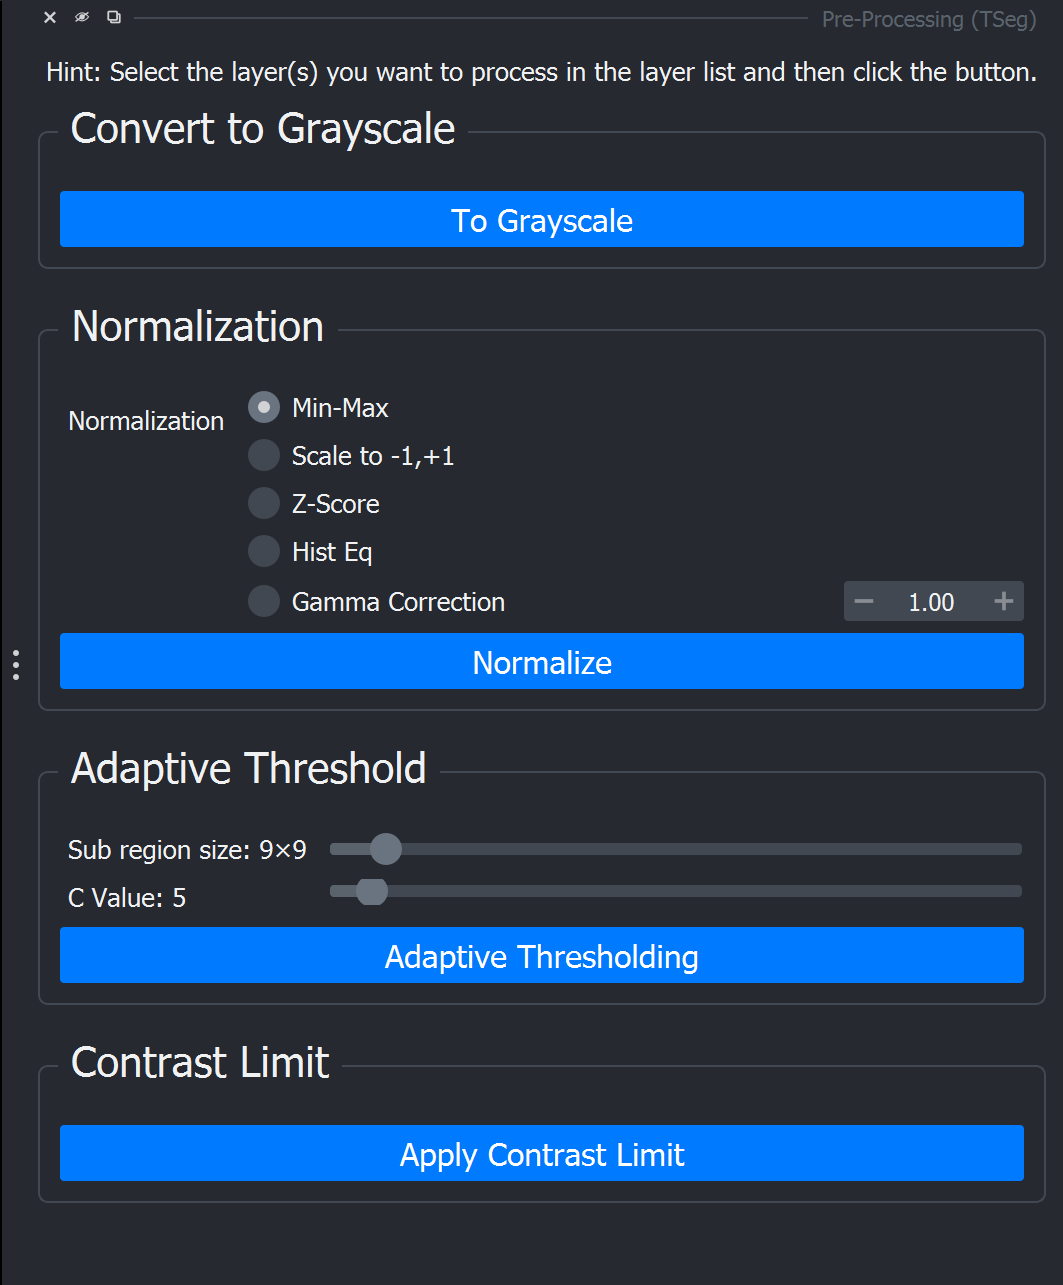
\includegraphics[width=.3\textwidth]{figures/tseg/pre widget.png}
    \caption{The pre-processing widget includes adaptive thresholding, normalization, and noise removal to enhance image quality.}
    \label{fig:preprocessing_widget}
\end{figure}


% \begin{figure}[h]
%     \centering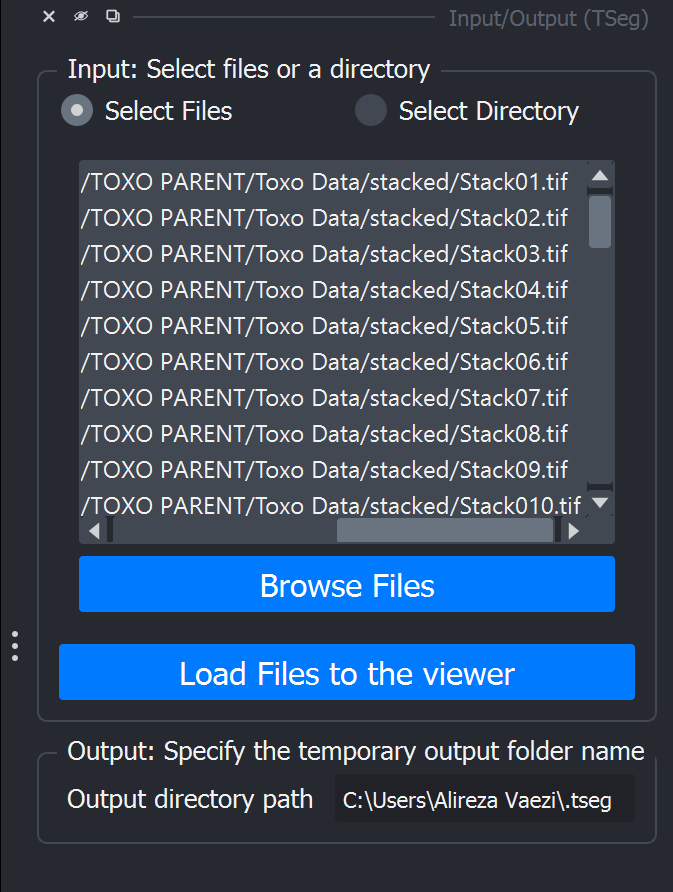
\includegraphics[width=.3\textwidth]{figures/tseg/io widget.png}
%     \caption{The IO widget consists of file management elements.}
%     \label{fig:io_widget}
% \end{figure}





\textbf{Cell Detection and Segmentation} \\
TSeg's Detection and Segmentation modules are in fact backed by PlantSeg and CellPose. The Detection Module is built only based on PlantSeg's CNN Detection Module \cite{plantseg}, and for the Segmentation Module, only one of the two tools can be selected to be executed as the segmentation tool in the pipeline. Naturally, each of the tools demands specific interface elements different from the others since each accepts different input values and various parameters. TSeg orchestrates this and makes sure the arguments and parameters are passed to the corresponding selected segmentation tool properly and the execution will be handled accordingly. The parameters include but are not limited to input data location, output directory, and desired segmentation algorithm - Figure \ref{fig:cnn_detection}. This allows the end-user complete control over the process and feedback from each step of the process. The preprocessed images and relevant parameters are sent to a modular segmentation controller script. As an effort to allow future development on TSeg, the segmentation controller script shows how the pipeline integrates two completely different segmentation packages.

\begin{figure}[h]
    \centering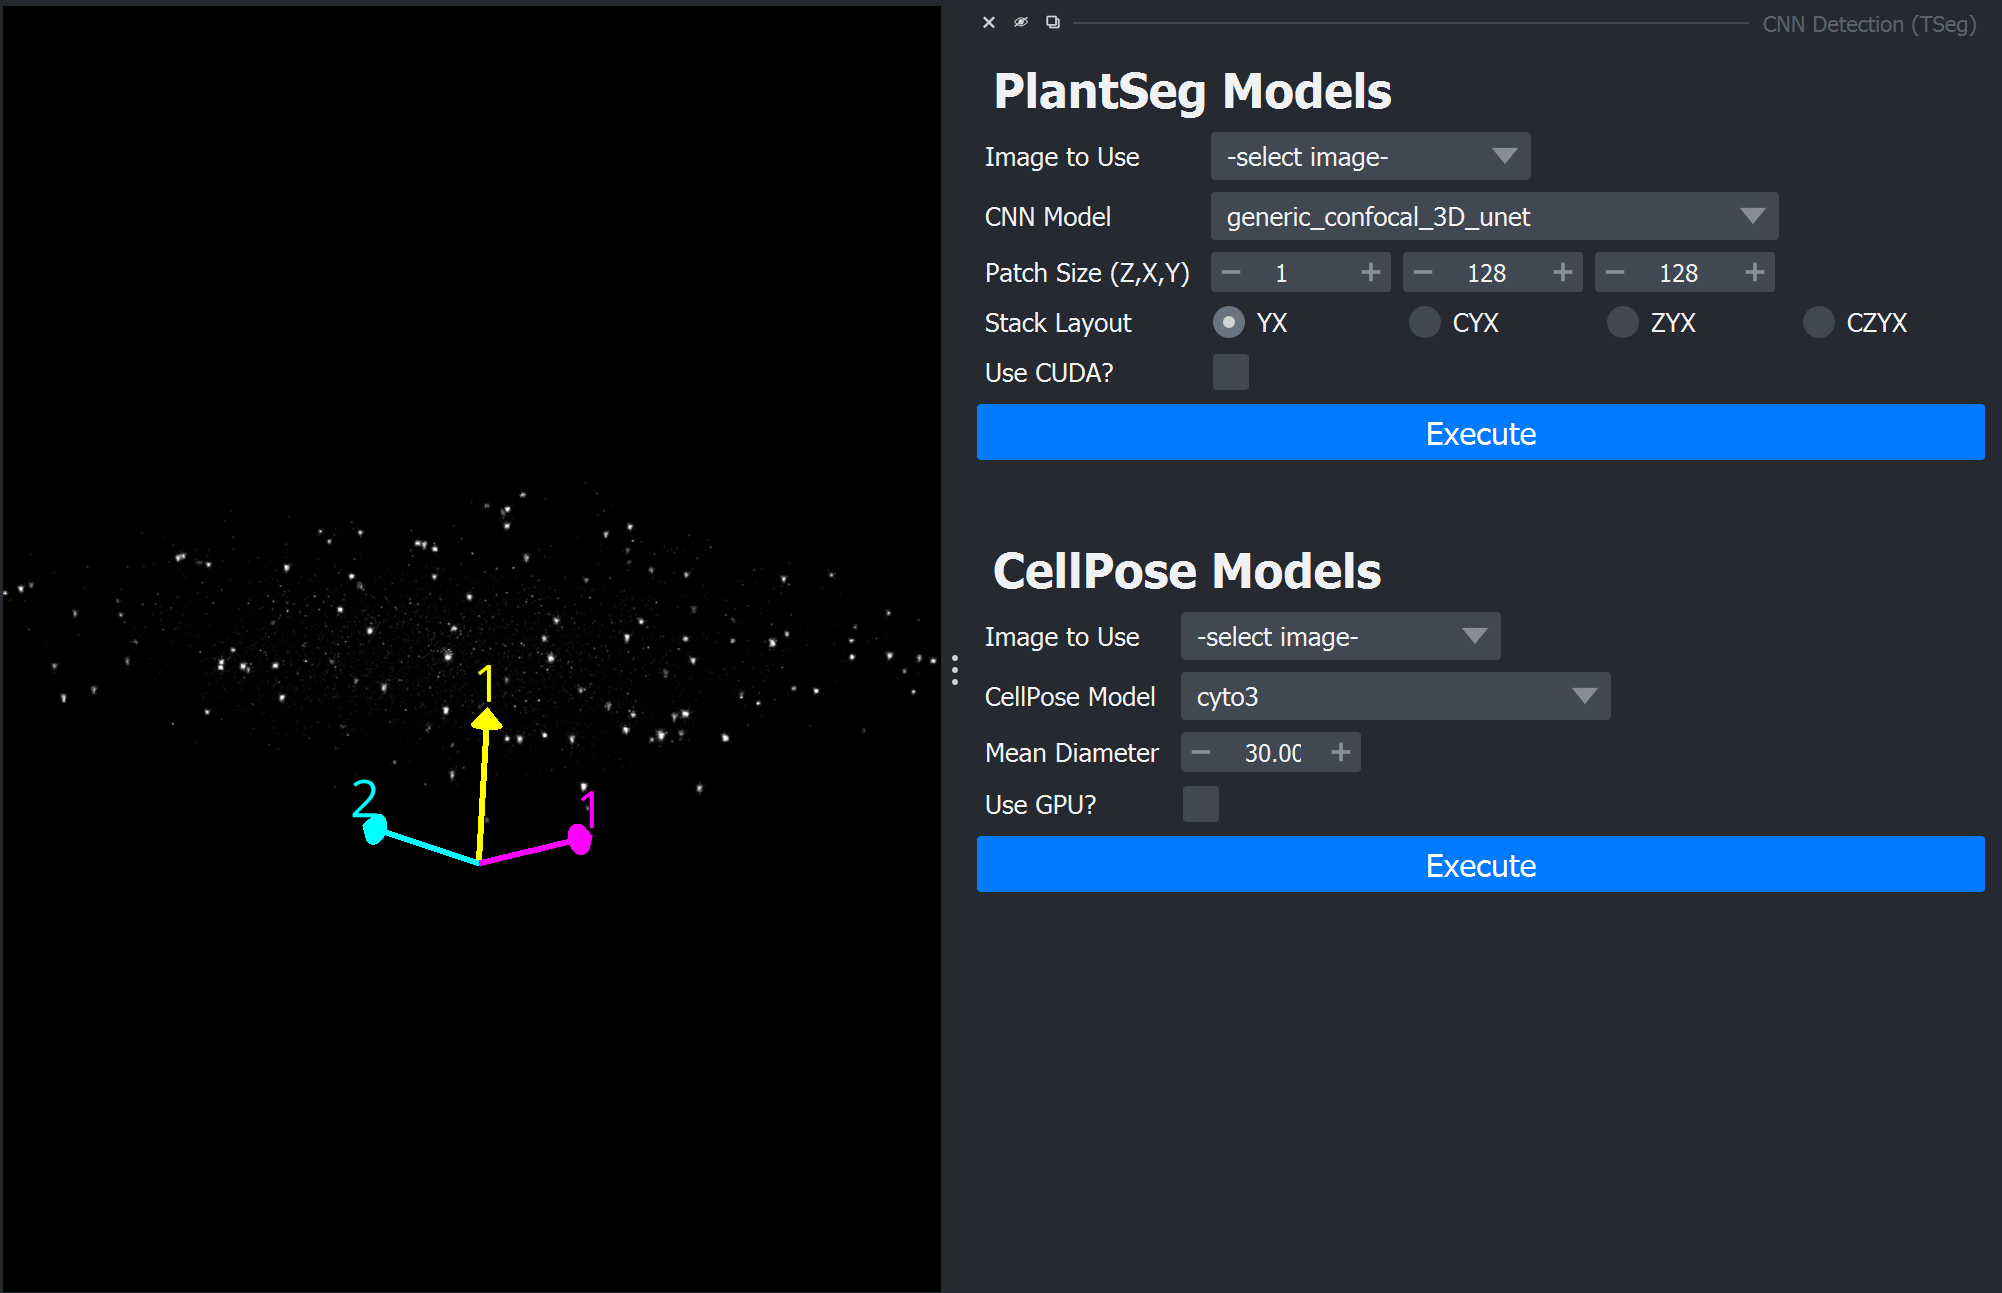
\includegraphics[width=.7\textwidth]{figures/tseg/cnn widget.png}
    \caption{The CNN Detection widget integrates PlantSeg for tissue-specific 3D segmentation and CellPose for diverse cell types. These tools are implemented in the backend via their APIs, ensuring seamless operation.}
    \label{fig:cnn_detection}
\end{figure}

\textbf{Tracking} \\
The tracking widget of TSeg employs connected component analysis and the Hungarian algorithm for accurate cell tracking across 3D time-lapse images,  and, leverages autoregressive modeling to analyze cell trajectories, enabling these trajectories to be clustered in an unsupervised manner for a deeper understanding of motility - Figure \ref{fig:tracking_widget}. Features in each segmented image are found using the scipy label function. In order to reduce any leftover noise, any features under a minimum size are filtered out and considered leftover noise. After feature extraction, centroids are calculated using the center of mass function in scipy. The centroid of the 3D cell can be used as a representation of the entire body during tracking. The tracking algorithm goes through each captured time instance and connects centroids to the likely next movement of the cell. Tracking involves a series of measures in order to avoid incorrect assignments. An incorrect assignment could lead to inaccurate result sets and unrealistic motility patterns. If the same number of features in each frame of time could be guaranteed from segmentation, minimum distance could assign features rather accurately. Since this is not a guarantee, the Hungarian algorithm must be used to associate a cost with the assignment of feature tracking. The Hungarian method is a combinatorial optimization algorithm that solves the assignment problem in polynomial time. The cost for the tracking algorithm determines which feature is the next iteration of the cell's tracking through the complete time series. The combination of distance between centroids for all previous points and the distance to the potential new centroid. If an optimal next centroid cannot be found within an acceptable distance of the current point, the tracking for the cell is considered as complete. Likewise, if a feature is not assigned to a current centroid, this feature is considered a new object and is tracked as the algorithm progresses. The complete path for each feature is then stored for motility analysis.
\begin{figure}[h]
    \centering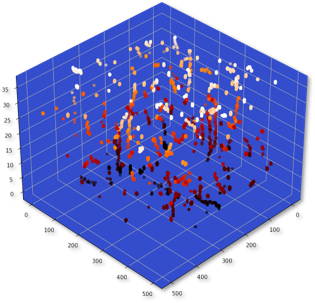
\includegraphics[width=.3\textwidth]{figures/tseg/centers.png}
    \centering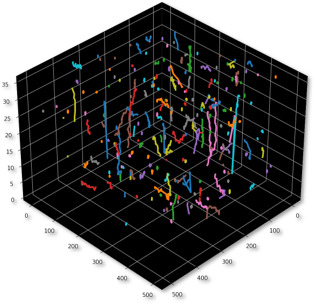
\includegraphics[width=.3\textwidth]{figures/tseg/tracking.png}
    \centering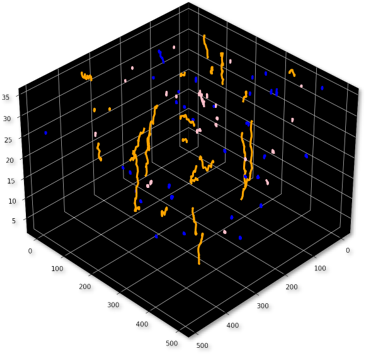
\includegraphics[width=.3\textwidth]{figures/tseg/trajs.png}
    \caption{Left, 3D connected component labeling (CCL) is used to extract features from the segmented images. Middle, the centroids of the features are calculated using the center of mass function in scipy. Right, the tracking algorithm connects centroids across time instances to track the cells.}
    \label{fig:tracking_plots}
\end{figure}
\begin{figure}[h]
    \centering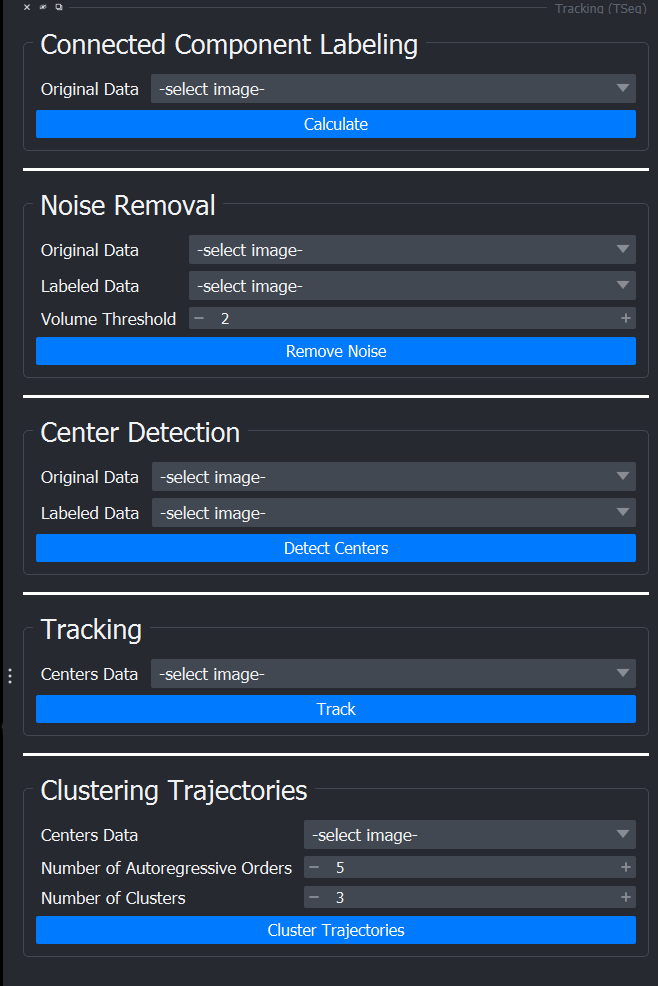
\includegraphics[width=.3\textwidth]{figures/tseg/tracking widget.png}
    \centering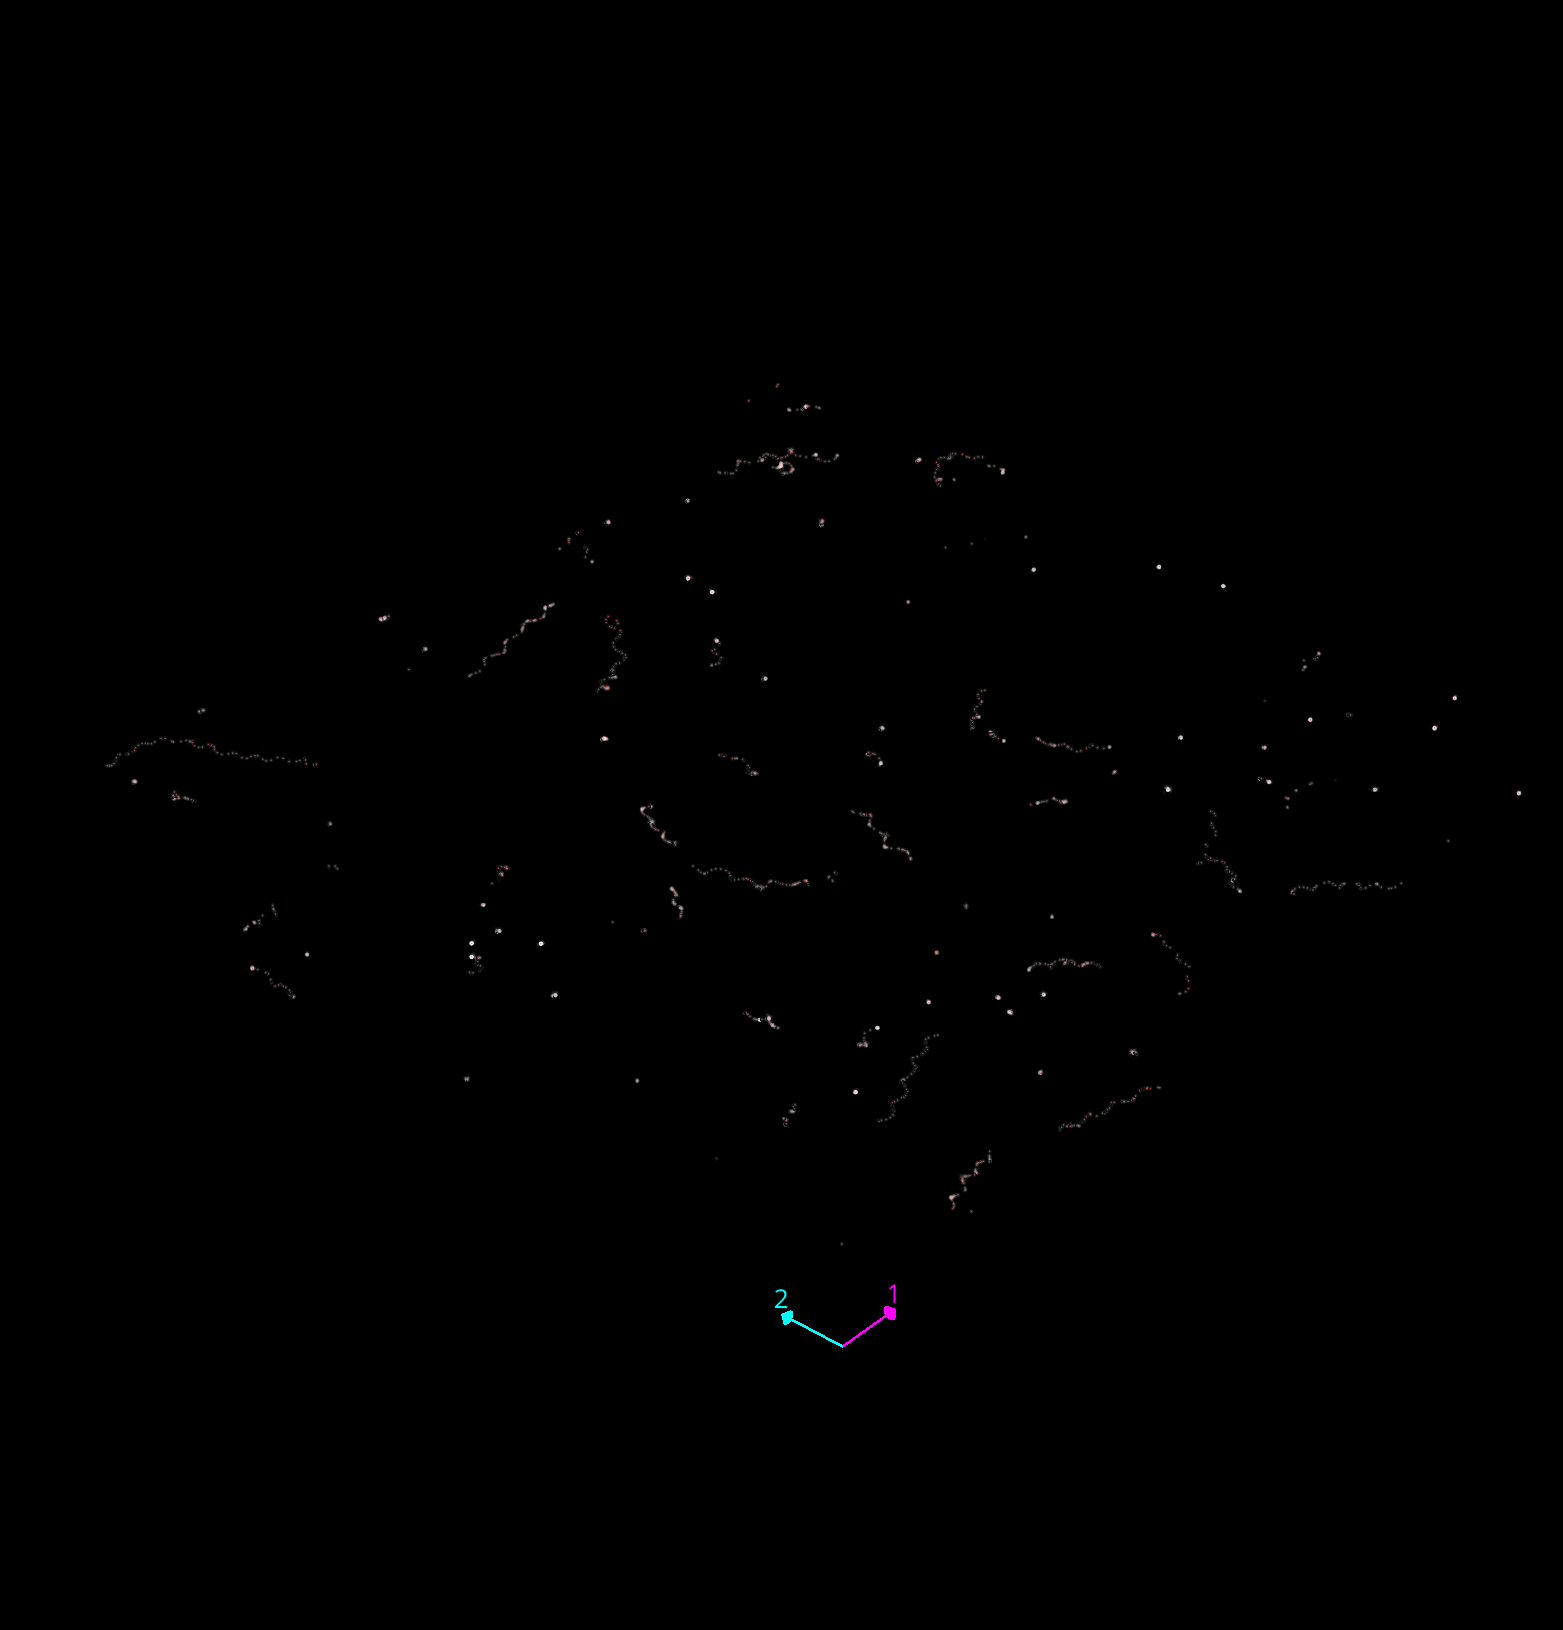
\includegraphics[width=.3\textwidth]{figures/tseg/tracking result.png}
    \centering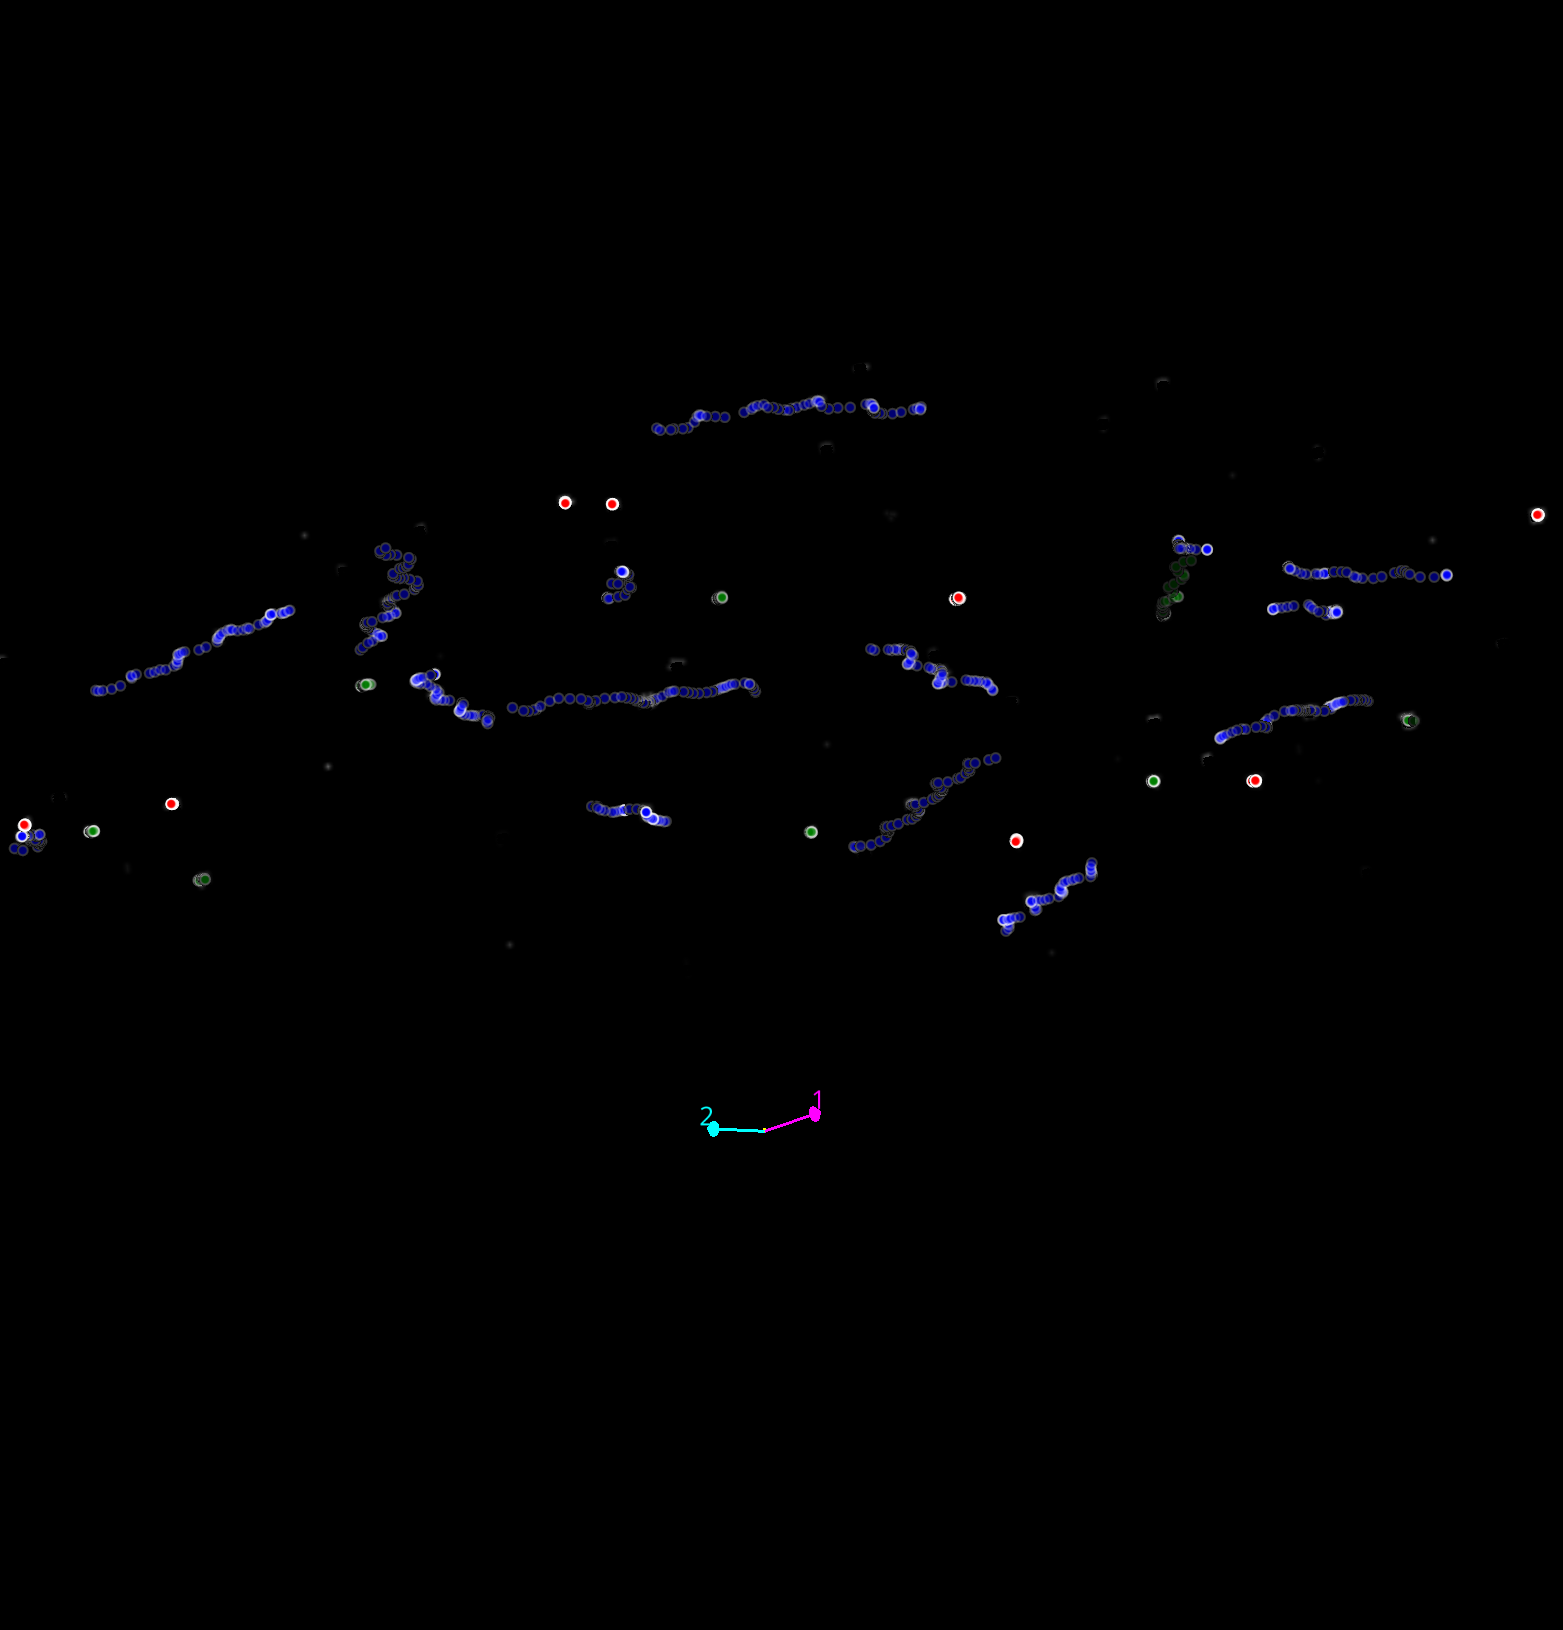
\includegraphics[width=.3\textwidth]{figures/tseg/clusters.png}
    \caption{The tracking widget allows the user to set the parameters for the tracking and clustering algorithms and visualizes the results.}
    \label{fig:tracking_widget}
\end{figure}


\textbf{Motion Classification} \\
To classify the motility pattern of \textit{\textit{T. gondii}} in 3D space in an unsupervised fashion we implement and use the method that Fazli et. al. introduced \cite{fazli2019lightweight}. In that work, they used an autoregressive model (AR); a linear dynamical system that encodes a Markov-based transition prediction method. The reason is that although K-means is a favorable clustering algorithm, there are a few drawbacks to it and to the conventional methods that draw them impractical. Firstly, K-means assumes Euclidian distance, but AR motion parameters are geodesics that do not reside in a Euclidean space, and secondly, K-means assumes isotropic clusters, however, although AR motion parameters may exhibit isotropy in their space, without a proper distance metric, this issue cannot be clearly examined \cite{fazli2019lightweight}.

\begin{figure}[h]
    \centering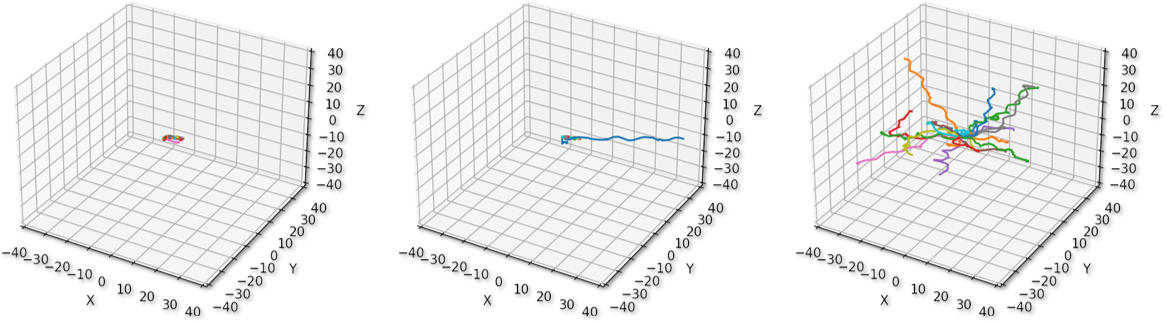
\includegraphics[width=.9\textwidth]{figures/tseg/clusters plot.png}
    \caption{Clustering of \textit{\textit{T. gondii}} motility patterns in 3D space using an autoregressive model (AR) as introduced by Fazli et al. \cite{fazli2019lightweight}. The AR model addresses the limitations of K-means by considering geodesic distances and non-isotropic clusters.}
    \label{fig:clustering}
\end{figure}

% Required packages in your preamble:
% \usepackage{graphicx} % To include images
% \usepackage{booktabs} % Optional: for better horizontal rules



\section{Evaluation}
TSeg's performance in segmentation was evaluated over datasets introduced in \cite{mavska2023cell}. The Cell Tracking Challenge (CTC) offers a diverse array of 2D and 3D time-lapse microscopy datasets, each capturing unique biological specimens under various imaging modalities. Table \ref{tbl:ctc_datasets} contains is an overview of these datasets, detailing the organisms studied, imaging techniques employed, and acquisition specifics. Table \ref{tab:ctc_datasets_visual_summary} shows a sample image of each dataset. CellPose has 26 and PlantSeg has 17 different pre-trained models that can perform segmentation over 2D and 3D biomedical data. 10 samples from the 2D datasets, and one from the 3D datasets were randomly selected and processed with each of the 43 models using the API provided by PlantSeg and CellPose. Each dataset contains sequences of time-lapse video frames, therefore sample of a 2D dataset is comprised of a single 2D grayscale image, and each sample from the 3D datasets has a stack of 2D images recorded simultaneously across the z-axis to comprise one frame. The predicted masks of the models were evaluated against the provided ground-truth data using the Jaccard Index (JI) score and averaged across all samples of the same dataset. The results of the best performing models of CellPose and PlantSeg are shown in Table \ref{tbl:best_2d_segmentation_summary} and Table \ref{tbl:best_3d_segmentation_summary} over 2D and 3D datasets respectively.

The JI scores of all models are available in the appendix. Tables~\ref{tbl:cellpose_2d_segmentation} and~\ref{tbl:plantseg_2d_segmentation} present the performance metrics for all CellPose and PlantSeg models on the 2D datasets. Tables~\ref{tbl:cellpose_3d_segmentation} and~\ref{tbl:plantseg_3d_segmentation} summarize their performance on the 3D datasets.

% {tbl:3d_segmentation_results}
\begin{table}[!ht]
    \centering
    \caption{Cell Tracking Challenge Datasets}
    \label{tbl:ctc_datasets}
    \renewcommand{\arraystretch}{1.3} % Adjust row spacing
    \small % Reduce font size
    \begin{tabular}{|l|p{2.3cm}|p{5cm}|p{2.3cm}|p{2.3cm}|}
        \hline
        \textbf{Dataset Name} & \textbf{Organism}       & \textbf{Description}                                                                                                        & \textbf{Imaging Modality}                           & \textbf{Dimension} \\ \hline
        BF-C2DL-HSC           & Mouse                   & Hematopoietic stem cells cultured in hydrogel microwells.                                                                   & Brightfield Microscopy                              & 2D                 \\ \hline
        BF-C2DL-MuSC          & Mouse                   & Muscle stem cells cultured in hydrogel microwells.                                                                          & Brightfield Microscopy                              & 2D                 \\ \hline
        DIC-C2DH-HeLa         & Human                   & HeLa cells cultured on a flat glass surface.                                                                                & Differential Interference Contrast (DIC) Microscopy & 2D                 \\ \hline
        Fluo-C2DL-Huh7        & Human                   & Huh7 cells expressing the fusion protein YFP-TIA-1.                                                                         & Fluorescence Microscopy                             & 2D                 \\ \hline
        Fluo-C2DL-MSC         & Rat                     & Mesenchymal stem cells cultured on a flat polyacrylamide substrate.                                                         & Fluorescence Microscopy                             & 2D                 \\ \hline
        Fluo-N2DH-GOWT1       & Mouse                   & GFP-GOWT1 stem cells.                                                                                                       & Fluorescence Microscopy                             & 2D                 \\ \hline
        Fluo-N2DL-HeLa        & Human                   & HeLa cells stably expressing H2b-GFP.                                                                                       & Fluorescence Microscopy                             & 2D                 \\ \hline
        Fluo-C3DH-A549        & Human                   & A549 lung cancer cells embedded in a Matrigel matrix.                                                                       & Fluorescence Microscopy                             & 3D                 \\ \hline
        Fluo-C3DH-H157        & Human                   & GFP-transfected H157 lung cancer cells embedded in a Matrigel matrix.                                                       & Fluorescence Microscopy                             & 3D                 \\ \hline
        Fluo-C3DL-MDA231      & Human                   & MDA231 human breast carcinoma cells infected with a pMSCV vector including the GFP sequence, embedded in a collagen matrix. & Fluorescence Microscopy                             & 3D                 \\ \hline
        Fluo-N3DH-CE          & C. elegans              & Developing C. elegans embryo.                                                                                               & Fluorescence Microscopy                             & 3D                 \\ \hline
        Fluo-N3DH-CHO         & Chinese Hamster         & Chinese Hamster Ovarian (CHO) nuclei overexpressing GFP-PCNA.                                                               & Fluorescence Microscopy                             & 3D                 \\ \hline
        Fluo-N3DL-DRO         & Drosophila melanogaster & Developing Drosophila melanogaster embryo.                                                                                  & Fluorescence Microscopy                             & 3D                 \\ \hline
        Fluo-N3DL-TRIC        & Tribolium castaneum     & Developing Tribolium castaneum embryo (3D cartographic projection).                                                         & Fluorescence Microscopy                             & 3D                 \\ \hline
        Fluo-N3DL-TRIF        & Tribolium castaneum     & Developing Tribolium castaneum embryo.                                                                                      & Fluorescence Microscopy                             & 3D                 \\ \hline
    \end{tabular}
\end{table}


CellPose demonstrated consistently strong performance across the majority of the evaluated 2D datasets, achieving accuracy levels often exceeding 0.90. Datasets like \textit{BF-C2DL-HSC}, \textit{BF-C2DL-MuSC}, and \textit{PhC-C2DL-PSC} showed particularly high segmentation accuracy, consistently surpassing 0.95. Notably, CellPose also maintained robust accuracy on diverse cell types and imaging modalities, indicating its effective generalization across different contexts.

PlantSeg, evaluated primarily on plant-based imaging datasets, showed impressive robustness and consistently high accuracy, especially for structured cellular patterns. On both 2D and 3D datasets, PlantSeg achieved similar high-performance metrics to CellPose, often with accuracy scores around 0.96 or higher.



\begin{table}[!ht]
    \centering
    \caption{Best Segmentation Performance on 2D CTC Datasets (Jaccard Index)}
    \label{tbl:best_2d_segmentation_summary}
    \renewcommand{\arraystretch}{1.2} % Adjust row spacing if needed
    \small % Reduce font size if needed
    \begin{tabular}{|l|l|c|l|c|}
        \hline
        \textbf{Dataset Name} & \textbf{JI (Best CellPose Model)}                 & \textbf{JI (Best PlantSeg Model)}                  \\ \hline
        BF-C2DL-HSC           & 0.99 (\texttt{nuclei / yeast\_BF\_cp3}\*        ) & 0.99 (\texttt{confocal\_2D\_unet\_ovules\_ds2x}\*) \\ \hline
        BF-C2DL-MuSC          & 0.99 (\texttt{nuclei / livecell\_cp3}\*         ) & 0.99 (\texttt{confocal\_2D\_unet\_ovules\_ds2x}\*) \\ \hline
        DIC-C2DH-HeLa         & 0.36 (\texttt{cyto3 / nuclei}\*                 ) & 0.36 (\texttt{confocal\_2D\_unet\_ovules\_ds2x}\*) \\ \hline
        Fluo-C2DL-Huh7        & 0.60 (\texttt{cyto3 / nuclei}\*                 ) & 0.59 (\texttt{confocal\_2D\_unet\_ovules\_ds2x}\*) \\ \hline
        Fluo-C2DL-MSC         & 0.90 (\texttt{cyto3 / cyto2}                    ) & 0.89 (\texttt{confocal\_2D\_unet\_ovules\_ds2x}\*) \\ \hline
        Fluo-N2DH-GOWT1       & 0.89 (\texttt{cyto3}                            ) & 0.86 (\texttt{confocal\_2D\_unet\_ovules\_ds2x}\*) \\ \hline
        Fluo-N2DH-SIM+        & 0.89 (\texttt{neurips\_grayscale\_cyto2}        ) & 0.80 (\texttt{confocal\_2D\_unet\_ovules\_ds2x}\*) \\ \hline
        Fluo-N2DL-HeLa        & 0.75 (\texttt{cyto3 / nuclei}\*                 ) & 0.75 (\texttt{confocal\_2D\_unet\_ovules\_ds2x}\*) \\ \hline
        PhC-C2DH-U373         & 0.87 (\texttt{cyto3 / nuclei}\*                 ) & 0.87 (\texttt{confocal\_2D\_unet\_ovules\_ds2x}\*) \\ \hline
        PhC-C2DL-PSC          & 0.91 (\texttt{tissuenet\_cp3 / livecell\_cp3}\* ) & 0.91 (\texttt{confocal\_2D\_unet\_ovules\_ds2x}\*) \\ \hline
    \end{tabular}
    % \caption*{\footnotesize \*Indicates multiple models achieved the same best score; one or two representatives are listed.}
\end{table}


However, during evaluation on 3D datasets, PlantSeg encountered challenges due to computational constraints. Several large-sized samples could not be fully processed by specific CNN architectures, resulting in incomplete results (indicated by blank cells in Table~\ref{tbl:plantseg_3d_segmentation}). This limitation primarily arose in datasets such as \textit{Fluo-N3DH-CE} and \textit{Fluo-N3DH-SIM+}, where the sheer volume of the input data surpassed the available computational resources, highlighting the computational demands associated with sophisticated 3D segmentation tasks. Future enhancements of PlantSeg may involve optimizing CNN architectures or leveraging computational strategies, such as tiling or cloud processing, to address these scalability limitations.


\begin{table}[!ht]
    \centering
    \caption{Best Segmentation Performance on 3D CTC Datasets (Jaccard Index)}
    \label{tbl:best_3d_segmentation_summary}
    \renewcommand{\arraystretch}{1.2} % Adjust row spacing if needed
    \small % Reduce font size if needed
    \begin{tabular}{|l|l|c|l|c|}
        \hline
        \textbf{Dataset Name} & \textbf{JI (Best CellPose Models)}        & \textbf{JI (Best PlantSeg Model)}                  \\ \hline
        Fluo-C3DH-A549        & 0.98 (\texttt{CPx, CP})                   & 0.96 ( \texttt{generic\_confocal\_3D\_unet}\*    ) \\ \hline
        Fluo-C3DH-A549-SIM    & 0.99 (\texttt{CPx, CP, TN3})              & 0.97 ( \texttt{generic\_confocal\_3D\_unet}\*    ) \\ \hline
        Fluo-C3DH-H157        & 0.93 (\texttt{cyto3, nuclei, cyto2\_cp3}) & 0.88 ( \texttt{generic\_confocal\_3D\_unet}\*    ) \\ \hline
        Fluo-N3DH-CE          & 0.80 (\texttt{cyto3, nuclei, cyto2\_cp3}) & 0.78 ( \texttt{generic\_confocal\_3D\_unet}\*\*  ) \\ \hline
        Fluo-N3DH-CHO         & 0.84 (\texttt{nuclei, tissuenet\_cp3 })   & 0.84 ( \texttt{generic\_confocal\_3D\_unet}\*    ) \\ \hline
        Fluo-N3DH-SIM+        & 0.94 (\texttt{cyto2})                     & ---  (   N/A (Processing failed)\*\*\*           ) \\ \hline
    \end{tabular}
    % \caption*{\footnotesize \*Indicates multiple PlantSeg models achieved the same best score; one representative listed. (\dots) indicates many CellPose models achieved the best score; only representative examples listed. \*\*Best score among PlantSeg models that successfully processed the data; some models failed due to computational constraints. \*\*\*All tested PlantSeg models failed on this dataset due to computational constraints.}
\end{table}


Overall, the evaluations demonstrate that both CellPose and PlantSeg effectively perform cell segmentation tasks across a range of datasets and conditions, with CellPose providing a slightly more versatile and robust generalization across various cell types and PlantSeg excelling particularly in structured datasets. Understanding these limitations and strengths will inform users' selection of the most appropriate tool based on their dataset characteristics and computational constraints. A comprehensive summary of segmentation performance metrics highlighting key comparative results between CellPose and PlantSeg on selected 2D and 3D datasets is presented in Tables~\ref{tbl:best_2d_segmentation_summary} and \ref{tbl:best_3d_segmentation_summary}. These tables succinctly capture essential findings, facilitating quick comparisons and reinforcing the suitability of TSeg's modular design in addressing diverse biomedical segmentation challenges. Furthermore, table \ref{tab:ctc_sota_top1_ji} provides the Jaccard Index of the top performing models from the Cell Tracking Challenge (CTC) 2023, showcasing the state-of-the-art performance of TSeg in comparison to other leading segmentation tools.



% % Master Table summarizing key segmentation results
% \begin{table}[!ht]
%     \centering
%     \caption{Comparative Summary of Segmentation Performance (Jaccard Index)}
%     \label{tbl:master_summary_segmentation}
%     \renewcommand{\arraystretch}{1.3}
%     \resizebox{\textwidth}{!}{
%         \begin{tabular}{|l|l|c|c|c|l|}
%             \hline
%             \textbf{Dataset Name} & \textbf{Imaging Modality} & \textbf{Dimension} & \textbf{Best CellPose Model (JI)} & \textbf{Best PlantSeg Model (JI)}                       & \textbf{Comments}                                                      \\ \hline
%             BF-C2DL-HSC           & Brightfield               & 2D                 & 0.99 (\texttt{livecell\_cp3})     & 0.99 (\texttt{confocal\_2D\_unet\_ovules\_ds2x})        & Excellent performance by both tools                                    \\ \hline
%             BF-C2DL-MuSC          & Brightfield               & 2D                 & 0.99 (\texttt{livecell\_cp3})     & 0.99 (\texttt{confocal\_2D\_unet\_ovules\_ds2x})        & Consistently high accuracy                                             \\ \hline
%             DIC-C2DH-HeLa         & DIC                       & 2D                 & 0.36 (\texttt{cyto3})             & 0.36 (\texttt{confocal\_2D\_unet\_sa\_meristem\_cells}) & Low accuracy due to imaging complexity                                 \\ \hline
%             Fluo-C2DL-MSC         & Fluorescence              & 2D                 & 0.90 (\texttt{cyto3})             & 0.89 (\texttt{confocal\_2D\_unet\_sa\_meristem\_cells}) & Good accuracy, slight advantage for CellPose                           \\ \hline
%             Fluo-N2DH-GOWT1       & Fluorescence              & 2D                 & 0.89 (\texttt{cyto3})             & 0.86 (\texttt{confocal\_2D\_unet\_sa\_meristem\_cells}) & Moderate accuracy, CellPose slightly better                            \\ \hline
%             Fluo-N2DL-HeLa        & Fluorescence              & 2D                 & 0.75 (\texttt{cyto3})             & 0.75 (\texttt{confocal\_2D\_unet\_sa\_meristem\_cells}) & Equal performance by both tools                                        \\ \hline
%             Fluo-C3DH-A549        & Fluorescence              & 3D                 & 0.98 (\texttt{CPx})               & 0.96 (\texttt{generic\_confocal\_3D\_unet})             & CellPose robust, strong performance by PlantSeg                        \\ \hline
%             Fluo-C3DH-H157        & Fluorescence              & 3D                 & 0.93 (\texttt{cyto3})             & 0.88 (\texttt{generic\_confocal\_3D\_unet})             & Higher robustness observed in CellPose                                 \\ \hline
%             Fluo-N3DH-CE          & Fluorescence              & 3D                 & 0.80 (\texttt{CPx})               & 0.78 (\texttt{generic\_confocal\_3D\_unet})             & Computationally challenging, slight CellPose advantage                 \\ \hline
%             Fluo-N3DH-CHO         & Fluorescence              & 3D                 & 0.84 (\texttt{CPx})               & 0.84 (\texttt{generic\_confocal\_3D\_unet})             & Similar results for both tools                                         \\ \hline
%             Fluo-N3DH-SIM+        & Fluorescence              & 3D                 & 0.94 (\texttt{cyto2})             & ---                                                     & Computationally intensive; PlantSeg failed due to resource constraints \\ \hline
%         \end{tabular}}
% \end{table}



% \subsection{Performance on 2D Datasets}

% The results show that segmentation performance varies significantly across datasets and models. Key observations include:
% \textbf{Consistently High Performance:} Models such as \texttt{cyto3}, \texttt{nuclei}, and \\ \texttt{deepbacs\_cp3} achieved high IoU scores (above 0.95) across datasets such as \texttt{BF-C2DL-HSC} and \texttt{BF-C2DL-MuSC}, which suggests that these models are well-suited for segmenting brightfield microscopy images of stem cells. \\

% \textbf{Challenges with Certain Datasets:} The \texttt{DIC-C2DH-HeLa} dataset posed difficulties for most models, with average IoU scores significantly lower (around 0.36), indicating that differential interference contrast (DIC) microscopy images present unique segmentation challenges. \\

% \textbf{Moderate Performance for Fluorescence-Based Data:} Models generally performed better on fluorescence microscopy datasets such as \texttt{Fluo-C2DL-MSC}, but the performance varied across different fluorescent markers and imaging conditions. \\

% \textbf{Model-Specific Variability:} While some models performed well across multiple datasets, others showed strong dataset-specific biases, highlighting the importance of dataset-matching when selecting segmentation models. \\

% \subsection{Performance on 3D Datasets \\}

% For the 3D datasets, the following trends emerged: \\

% \textbf{Superior Performance on Some Fluorescence Datasets:} Models like \texttt{PlantSeg\_3Dnuc\_platinum} and \texttt{lightsheet\_3D\_unet\_root\_ds2x} demonstrated high performance (IoU $\sim$0.96--0.97) on \texttt{Fluo-C3DH-A549} and \texttt{Fluo-C3DH-A549-SIM}, suggesting strong adaptability to fluorescence-based 3D segmentation. \\

% \textbf{Lower Performance on More Complex 3D Structures:} Datasets such as Fluo-N3DH-CE and Fluo-N3DH-CHO showed lower overall IoU scores, with some models failing to generalize well to these samples. \\

% \textbf{Sparse Data and Missing Values:} Several models had missing scores for certain datasets, indicating either difficulties in processing specific images or incompatibility with the dataset structure. \\


% Required packages in your preamble:
% \usepackage{booktabs} % for better rules (\toprule, \midrule, \bottomrule)
% \usepackage{rotating} % for \rotatebox

\begin{table}[h] % 'htbp' suggests placement options: here, top, bottom, page
    \centering
    \caption{Top-Performing Jaccard Index Scores on 2D CTC Datasets.} % Updated caption
    \label{tab:ctc_sota_top1_ji} % Updated label
    % \small % Adjust font size if needed
    \begin{tabular}{|l|c|} % 2 columns: Left-aligned text, Right-aligned number
        \hline
        Dataset/Metric   & Jaccard Index \\ \hline
        BF-C2DL-HSC      & 0.895         \\ \hline
        BF-C2DL-MuSC     & 0.784         \\ \hline
        DIC-C2DH-HeLa    & 0.871         \\ \hline
        Fluo-C2DL-Huh7   & 0.811         \\ \hline
        Fluo-C2DL-MSC    & 0.687         \\ \hline
        Fluo-N2DH-GOWT1  & 0.938         \\ \hline
        Fluo-N2DL-HeLa   & 0.913         \\ \hline
        PhC-C2DH-U373    & 0.931         \\ \hline
        PhC-C2DL-PSC     & 0.756         \\ \hline
        Fluo-C3DH-A549   & 0.908         \\ \hline
        Fluo-C3DH-H157   & 0.890         \\ \hline
        Fluo-C3DL-MDA231 & 0.710         \\ \hline
        Fluo-N3DH-CE     & 0.759         \\ \hline
        Fluo-N3DH-CHO    & 0.925         \\ \hline
        Fluo-N3DL-DRO    & 0.760         \\ \hline
        Fluo-N3DL-TRIC   & 0.821         \\ \hline
        Fluo-N3DL-TRIF   & 0.793         \\ \hline
    \end{tabular}
    % Optional notes below the table
    % \begin{tablenotes}
    %     \item[*] Note: Asterisk indicates ... (explain if necessary, e.g., specific challenge version or if the score itself is notable)
    % \end{tablenotes}
\end{table}


\section{Conclusion and Final Remarks}
% TSeg is an easy to use pipeline designed to study the motility patterns of \textit{\textit{T. gondii}} in 3D space. It is developed as a plugin for Napari and is equipped with a variety of deep learning based segmentation tools borrowed from PlantSeg and CellPose, making it a suitable off-the-shelf tool for applications incorporating images of cell types not limited to \textit{\textit{T. gondii}}. Future work on TSeg includes the expansion of implemented algorithms and tools in its preprocessing, segmentation, tracking, and clustering modules.

In this work, we presented TSeg, an intuitive and comprehensive pipeline specifically designed for the segmentation, tracking, and motility clustering of \textit{Toxoplasma gondii} in 3D microscopic imaging data. Our pipeline leverages autoregressive parameterization to effectively capture temporal dependencies, successfully identifying distinct motility patterns and accurately clustering them based on their inherent characteristics. This approach provides insights into the complex motility behavior exhibited by \textit{T. gondii} throughout its lytic cycle, facilitating more detailed and quantitative analyses compared to conventional methods.

One of the key contributions of our work is the seamless integration of state-of-the-art deep learning methodologies into an accessible and user-friendly platform. By incorporating powerful segmentation and detection tools such as CellPose and PlantSeg into TSeg, users benefit from high-performing deep learning algorithms without requiring extensive expertise in deep learning or computer vision frameworks. Additionally, our implementation of TSeg as a plugin for the Napari viewer further simplifies its adoption, providing interactive visualization and intuitive manipulation of 3D microscopy data.

TSeg significantly enhances the daily workflow of biological researchers by democratizing the analysis of complex 3D microscopic image data, making sophisticated quantitative studies accessible even to users without deep learning or extensive programming knowledge. Its implementation as a Napari plugin provides an intuitive graphical interface featuring immediate 3D visualization and feedback at each stage, allowing users to iteratively refine parameters and evaluate intermediate results. This user-centric design, combined with powerful underlying algorithms leveraging state-of-the-art tools like CellPose and PlantSeg, substantially improves the speed and quality of cell segmentation and tracking compared to manual methods or pipelines requiring extensive customization, directly addressing the challenges of time-consuming and expertise-heavy analysis.

Furthermore, TSeg functions as an adhesive component within the broader open-source scientific ecosystem. Built upon the familiar SciPy stack and integrated directly into Napari, its utility extends beyond its initial focus on \textit{T. gondii}, proving adaptable to various other cell types and organisms. Its development exemplifies open-science principles through its open-source availability and reliance on well-regarded packages, aligning with the collaborative spirit fostered by communities such as PyOpenSci and the Journal of Open Source Software (JOSS). Looking forward, continuous enhancements in computational efficiency and scalability are envisioned to further broaden TSeg's usability across larger and more complex datasets, ultimately fulfilling its significant potential to accelerate biological research by making advanced analyses readily available to a wider scientific audience.


\section{Limitations and Future Directions}
While TSeg provides an intuitive and integrated pipeline for 3D cell analysis, several limitations should be acknowledged.

\textbf{Limitations of TSeg:}
\begin{itemize}
    \item Its performance can face computational constraints when processing large 3D datasets. This is particularly true when utilizing integrated tools like PlantSeg, which sometimes encountered memory limitations on complex CTC samples. Consequently, TSeg's overall accuracy is inherently linked to the performance and limitations of the specific tools it incorporates, namely PlantSeg and CellPose.

    \item The tracking module, relying on centroid calculation and the Hungarian algorithm, may encounter difficulties with complex cellular events such as division, fusion, or temporary occlusion. This could potentially lead to assignment errors in dense or highly dynamic scenarios.

    \item  Although designed with generic functions and evaluated on various cell types, TSeg was initially developed focusing on \textit{T. gondii}. Its effectiveness might therefore vary on significantly different cell types or imaging modalities not covered in the evaluations, requiring further validation for broader generalization.

    \item Furthermore, the motility classification employs an AR model which might not capture the full complexity of diverse biological movement patterns observed in different cell types or conditions.

    \item  Finally, while the preprocessing module addresses common artifacts like vignetting and noise, it may not encompass all specific artifacts encountered in varied microscopy setups, potentially necessitating external preprocessing steps for optimal results.

\end{itemize}
\textbf{Future Directions:}
\begin{itemize}
    \item Addressing the computational bottlenecks to improve scalability and efficiency, especially for large 3D time-lapse datasets, is a key priority for future development. This could involve optimizing existing algorithms or exploring strategies like data tiling.

    \item Expanding the repertoire of integrated segmentation and tracking algorithms beyond CellPose and PlantSeg can offer users greater flexibility. Incorporating more diverse algorithms could provide potentially improved performance tailored to specific biological contexts or challenging imaging conditions.

    \item Enhancing the robustness of the tracking algorithm is crucial for broader applicability. Future work should focus on better handling complex events like high cell density, cell division, fusion events, and temporary disappearance or occlusion of cells, perhaps exploring alternative tracking paradigms. Improving the tracking module could enable TSeg to handle more complex scenarios, such as mitochondrial dynamics or cell-cell interactions, which are common in biological systems.

    \item Advancing the motion classification module by exploring non-linear models or alternative machine learning approaches could provide deeper insights into complex motility phenotypes beyond the capabilities of the current AR model. Furthermore, exploring the spectrum of motion of parameterized trajectories could yield valuable insights into the underlying biological processes if a true correspondance between the motility phenotypes and the motion manifold is established.

    \item More extensive validation of TSeg's generalizability across a wider range of 3D cell types, organisms, and imaging modalities is needed to better define its scope and reliability in diverse research settings.

    \item Integrating TSeg's outputs seamlessly with downstream quantitative analysis tools would facilitate more comprehensive biological investigations, allowing researchers to easily move from segmentation and tracking to deeper statistical analysis.

    \item Lastly, incorporating mechanisms for user-guided refinement within the Napari interface could improve usability. Allowing users to interactively correct segmentation or tracking results would be particularly beneficial in ambiguous or challenging cases.
\end{itemize}

\end{document}
